\documentclass{article}
\usepackage{amsmath}
\usepackage{amssymb}
\usepackage{graphicx}
\usepackage{hyperref}
\usepackage[version=4]{mhchem}

\title{Problem 4}
\date{}

\begin{document}
\maketitle

\section*{Problem}
( \(A M C\) ) In the obtuse triangle \(A B C, A M=M B, M D \perp B C, E C \perp B C\). If the area of \(\triangle A B C\) is 24 , find the area of \(\triangle B E D\).\\
\centering
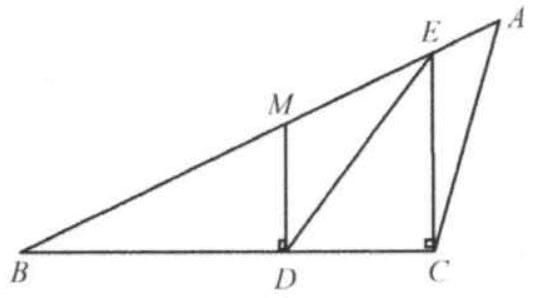
\includegraphics[width=\textwidth]{images/015.jpg}

\section*{Solution}
12.
Draw the median MC (Figure 1).\\
Since \(M D\) and \(E C\) are parallel, the colored areas in Figure 2 are the same. The area of \(\triangle B E D\) is the same as the area of \(\triangle B M C\) (Figure 3), which is half of the area of \(\triangle A B C\). The answer is \(24 / 2=12\).\\
\centering
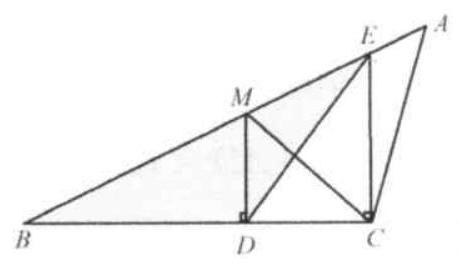
\includegraphics[width=\textwidth]{images/018(2).jpg}

Figure 1\\
\centering
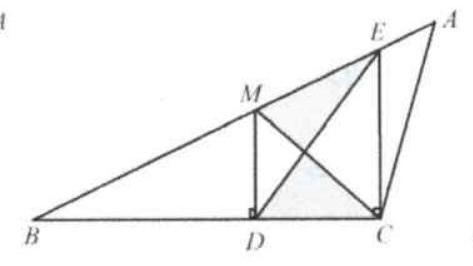
\includegraphics[width=\textwidth]{images/018.jpg}

Figure 2\\
\centering
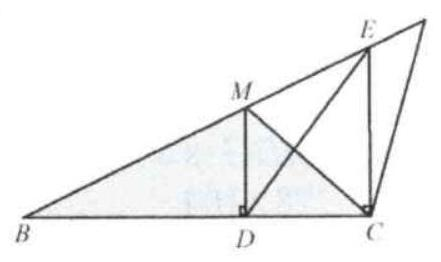
\includegraphics[width=\textwidth]{images/018(1).jpg}

Figure 3

\end{document}
